\documentclass[twoside]{book}

% Packages required by doxygen
\usepackage{fixltx2e}
\usepackage{calc}
\usepackage{doxygen}
\usepackage[export]{adjustbox} % also loads graphicx
\usepackage{graphicx}
\usepackage[utf8]{inputenc}
\usepackage{makeidx}
\usepackage{multicol}
\usepackage{multirow}
\PassOptionsToPackage{warn}{textcomp}
\usepackage{textcomp}
\usepackage[nointegrals]{wasysym}
\usepackage[table]{xcolor}

% Font selection
\usepackage[T1]{fontenc}
\usepackage[scaled=.90]{helvet}
\usepackage{courier}
\usepackage{amssymb}
\usepackage{sectsty}
\renewcommand{\familydefault}{\sfdefault}
\allsectionsfont{%
  \fontseries{bc}\selectfont%
  \color{darkgray}%
}
\renewcommand{\DoxyLabelFont}{%
  \fontseries{bc}\selectfont%
  \color{darkgray}%
}
\newcommand{\+}{\discretionary{\mbox{\scriptsize$\hookleftarrow$}}{}{}}

% Page & text layout
\usepackage{geometry}
\geometry{%
  a4paper,%
  top=2.5cm,%
  bottom=2.5cm,%
  left=2.5cm,%
  right=2.5cm%
}
\tolerance=750
\hfuzz=15pt
\hbadness=750
\setlength{\emergencystretch}{15pt}
\setlength{\parindent}{0cm}
\setlength{\parskip}{3ex plus 2ex minus 2ex}
\makeatletter
\renewcommand{\paragraph}{%
  \@startsection{paragraph}{4}{0ex}{-1.0ex}{1.0ex}{%
    \normalfont\normalsize\bfseries\SS@parafont%
  }%
}
\renewcommand{\subparagraph}{%
  \@startsection{subparagraph}{5}{0ex}{-1.0ex}{1.0ex}{%
    \normalfont\normalsize\bfseries\SS@subparafont%
  }%
}
\makeatother

% Headers & footers
\usepackage{fancyhdr}
\pagestyle{fancyplain}
\fancyhead[LE]{\fancyplain{}{\bfseries\thepage}}
\fancyhead[CE]{\fancyplain{}{}}
\fancyhead[RE]{\fancyplain{}{\bfseries\leftmark}}
\fancyhead[LO]{\fancyplain{}{\bfseries\rightmark}}
\fancyhead[CO]{\fancyplain{}{}}
\fancyhead[RO]{\fancyplain{}{\bfseries\thepage}}
\fancyfoot[LE]{\fancyplain{}{}}
\fancyfoot[CE]{\fancyplain{}{}}
\fancyfoot[RE]{\fancyplain{}{\bfseries\scriptsize 制作者 Doxygen }}
\fancyfoot[LO]{\fancyplain{}{\bfseries\scriptsize 制作者 Doxygen }}
\fancyfoot[CO]{\fancyplain{}{}}
\fancyfoot[RO]{\fancyplain{}{}}
\renewcommand{\footrulewidth}{0.4pt}
\renewcommand{\chaptermark}[1]{%
  \markboth{#1}{}%
}
\renewcommand{\sectionmark}[1]{%
  \markright{\thesection\ #1}%
}

% Indices & bibliography
\usepackage{natbib}
\usepackage[titles]{tocloft}
\setcounter{tocdepth}{3}
\setcounter{secnumdepth}{5}
\makeindex

% Custom commands
\newcommand{\clearemptydoublepage}{%
  \newpage{\pagestyle{empty}\cleardoublepage}%
}

\usepackage{caption}
\captionsetup{labelsep=space,justification=centering,font={bf},singlelinecheck=off,skip=4pt,position=top}

%===== C O N T E N T S =====

\begin{document}

% Titlepage & ToC
\pagenumbering{roman}
\begin{titlepage}
\vspace*{7cm}
\begin{center}%
{\Large Miniword \\[1ex]\large 0.\+0 }\\
\vspace*{1cm}
{\large 制作者 Doxygen 1.8.11}\\
\end{center}
\end{titlepage}
\clearemptydoublepage
\tableofcontents
\clearemptydoublepage
\pagenumbering{arabic}

%--- Begin generated contents ---
\chapter{概要设计}
\label{index}\section{Introduction}\label{index_intro_sec}
This is the introduction.\section{Installation}\label{index_install_sec}
\subsection{Step 1\+: Opening the box}\label{index_step1}
etc... 
\chapter{继承关系索引}
\section{类继承关系}
此继承关系列表按字典顺序粗略的排序\+: \begin{DoxyCompactList}
\item Q\+Frame\begin{DoxyCompactList}
\item \contentsline{section}{H\+Paint\+Area}{\pageref{class_h_paint_area}}{}
\end{DoxyCompactList}
\item Q\+Main\+Window\begin{DoxyCompactList}
\item \contentsline{section}{Main\+Window}{\pageref{class_main_window}}{}
\end{DoxyCompactList}
\item Q\+Object\begin{DoxyCompactList}
\item \contentsline{section}{H\+Document\+Model}{\pageref{class_h_document_model}}{}
\item \contentsline{section}{H\+Render\+Controller}{\pageref{class_h_render_controller}}{}
\end{DoxyCompactList}
\item Q\+Widget\begin{DoxyCompactList}
\item \contentsline{section}{H\+Text\+Cursor}{\pageref{class_h_text_cursor}}{}
\end{DoxyCompactList}
\end{DoxyCompactList}

\chapter{类索引}
\section{类列表}
这里列出了所有类、结构、联合以及接口定义等,并附带简要说明\+:\begin{DoxyCompactList}
\item\contentsline{section}{{\bf H\+Document\+Model} }{\pageref{class_h_document_model}}{}
\item\contentsline{section}{{\bf H\+Paint\+Area} }{\pageref{class_h_paint_area}}{}
\item\contentsline{section}{{\bf H\+Render\+Controller} }{\pageref{class_h_render_controller}}{}
\item\contentsline{section}{{\bf H\+Text\+Cursor} }{\pageref{class_h_text_cursor}}{}
\item\contentsline{section}{{\bf Main\+Window} }{\pageref{class_main_window}}{}
\end{DoxyCompactList}

\chapter{类说明}
\section{H\+Document\+Model类 参考}
\label{class_h_document_model}\index{H\+Document\+Model@{H\+Document\+Model}}


类 H\+Document\+Model 继承关系图\+:\nopagebreak
\begin{figure}[H]
\begin{center}
\leavevmode
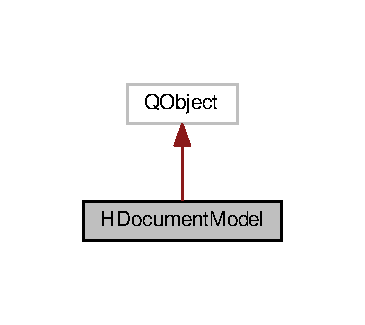
\includegraphics[width=175pt]{class_h_document_model__inherit__graph}
\end{center}
\end{figure}


H\+Document\+Model 的协作图\+:\nopagebreak
\begin{figure}[H]
\begin{center}
\leavevmode
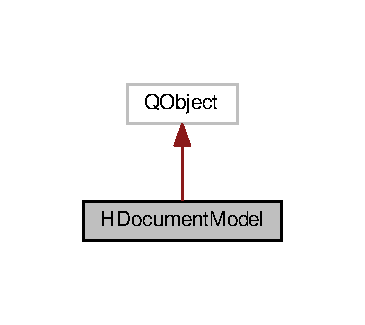
\includegraphics[width=175pt]{class_h_document_model__coll__graph}
\end{center}
\end{figure}
\subsection*{Public 类型}
\begin{DoxyCompactItemize}
\item 
enum {\bf Model\+Status} \{ {\bfseries H\+L\+L\+No\+Change}, 
{\bfseries H\+L\+L\+Updated}, 
{\bfseries H\+L\+L\+Created}, 
{\bfseries H\+L\+L\+Deleted}
 \}\label{class_h_document_model_a225db78eec58aaaeb20421332287588c}
\begin{DoxyCompactList}\small\item\em Model层状态枚举类型 \end{DoxyCompactList}
\end{DoxyCompactItemize}
\subsection*{信号}
\begin{DoxyCompactItemize}
\item 
void {\bfseries model\+Changed} ()\label{class_h_document_model_abf501351e0a321861ccb4c2b20f4df24}

\end{DoxyCompactItemize}
\subsection*{Public 成员函数}
\begin{DoxyCompactItemize}
\item 
Q\+List$<$ char $\ast$ $>$ \& {\bf create\+Logic\+Line} (Q\+String Line, int pos)
\item 
Q\+List$<$ char $\ast$ $>$ \& {\bf create\+Logic\+Line} (Q\+String Line)
\begin{DoxyCompactList}\small\item\em 重载类型 \end{DoxyCompactList}\item 
Q\+Shared\+Pointer$<$ Q\+String $>$ {\bf compose\+Logic\+Line} (int row) const 
\item 
void {\bf delete\+Logic\+Linek} (int pos)
\begin{DoxyCompactList}\small\item\em 删除逻辑行 \end{DoxyCompactList}\item 
void {\bf ensure\+Status} (int pos, {\bf Model\+Status} type)
\begin{DoxyCompactList}\small\item\em 重置\+Model层状态 \end{DoxyCompactList}\end{DoxyCompactItemize}


\subsection{详细描述}


在文件 hdocumentmodel.\+h 第 10 行定义.



\subsection{成员函数说明}
\index{H\+Document\+Model@{H\+Document\+Model}!compose\+Logic\+Line@{compose\+Logic\+Line}}
\index{compose\+Logic\+Line@{compose\+Logic\+Line}!H\+Document\+Model@{H\+Document\+Model}}
\subsubsection[{compose\+Logic\+Line(int row) const }]{\setlength{\rightskip}{0pt plus 5cm}Q\+Shared\+Pointer$<$ Q\+String $>$ H\+Document\+Model\+::compose\+Logic\+Line (
\begin{DoxyParamCaption}
\item[{int}]{row}
\end{DoxyParamCaption}
) const}\label{class_h_document_model_a9f99da8f5105c71c69acc22811c9c9dd}

\begin{DoxyParams}{参数}
{\em row} & 逻辑行的行数 \\
\hline
\end{DoxyParams}
\begin{DoxyReturn}{返回}
指向\+Q\+String 对象的指针
\end{DoxyReturn}
我将一个逻辑行内的对象复合成一个\+Q\+String类型。如果行数超出了范围,则返回一个空指针。 

在文件 hdocumentmodel.\+cpp 第 42 行定义.

\index{H\+Document\+Model@{H\+Document\+Model}!create\+Logic\+Line@{create\+Logic\+Line}}
\index{create\+Logic\+Line@{create\+Logic\+Line}!H\+Document\+Model@{H\+Document\+Model}}
\subsubsection[{create\+Logic\+Line(\+Q\+String Line, int pos)}]{\setlength{\rightskip}{0pt plus 5cm}Q\+List$<$ char $\ast$ $>$ \& H\+Document\+Model\+::create\+Logic\+Line (
\begin{DoxyParamCaption}
\item[{Q\+String}]{Line, }
\item[{int}]{pos}
\end{DoxyParamCaption}
)}\label{class_h_document_model_aaa2580ec2adcaf6a31f32436afbbcf57}

\begin{DoxyParams}{参数}
{\em Line} & 要添加到该逻辑行的字符串 \\
\hline
{\em pos} & 新逻辑行将作为文档的第pos行。(从0行开始算起) \\
\hline
\end{DoxyParams}
\begin{DoxyReturn}{返回}
指向新插入行的引用类型
\end{DoxyReturn}
添加新逻辑行.\+使用要求的数据结构存储数据。 pos如果大于当前的逻辑行数,新插入的行将作为最后一行。 pos如果为负,新插入的行作为首行。 保持状态同步 

在文件 hdocumentmodel.\+cpp 第 17 行定义.

\index{H\+Document\+Model@{H\+Document\+Model}!create\+Logic\+Line@{create\+Logic\+Line}}
\index{create\+Logic\+Line@{create\+Logic\+Line}!H\+Document\+Model@{H\+Document\+Model}}
\subsubsection[{create\+Logic\+Line(\+Q\+String Line)}]{\setlength{\rightskip}{0pt plus 5cm}Q\+List$<$ char $\ast$ $>$ \& H\+Document\+Model\+::create\+Logic\+Line (
\begin{DoxyParamCaption}
\item[{Q\+String}]{Line}
\end{DoxyParamCaption}
)}\label{class_h_document_model_af4a0fc68a7437bf81873be7bc333ff50}


重载类型 


\begin{DoxyParams}{参数}
{\em Line} & 要添加到该逻辑行的字符串 \\
\hline
\end{DoxyParams}
\begin{DoxyReturn}{返回}
指向新插入行的引用类型
\end{DoxyReturn}
我是为 \doxyref{create\+Logic\+Line(\+Q\+String,int)}{p.}{class_h_document_model_aaa2580ec2adcaf6a31f32436afbbcf57} 的重载类型。使用我直接在最后一行处插入\+Logic Line 

在文件 hdocumentmodel.\+cpp 第 36 行定义.

\index{H\+Document\+Model@{H\+Document\+Model}!delete\+Logic\+Linek@{delete\+Logic\+Linek}}
\index{delete\+Logic\+Linek@{delete\+Logic\+Linek}!H\+Document\+Model@{H\+Document\+Model}}
\subsubsection[{delete\+Logic\+Linek(int pos)}]{\setlength{\rightskip}{0pt plus 5cm}void H\+Document\+Model\+::delete\+Logic\+Linek (
\begin{DoxyParamCaption}
\item[{int}]{pos}
\end{DoxyParamCaption}
)}\label{class_h_document_model_a83cde52b7951fcd8bd604df255f9b5c1}


删除逻辑行 


\begin{DoxyParams}{参数}
{\em pos} & 删除当前第pos行,从0开始计算。\\
\hline
\end{DoxyParams}
pos应当对应一个客观存在的逻辑行位置。 (0 $<$= pos $<$ max\+Line) 如果pos不对应任何行,那么将没有任何东西被删除。 \index{H\+Document\+Model@{H\+Document\+Model}!ensure\+Status@{ensure\+Status}}
\index{ensure\+Status@{ensure\+Status}!H\+Document\+Model@{H\+Document\+Model}}
\subsubsection[{ensure\+Status(int pos, Model\+Status type)}]{\setlength{\rightskip}{0pt plus 5cm}void H\+Document\+Model\+::ensure\+Status (
\begin{DoxyParamCaption}
\item[{int}]{pos, }
\item[{{\bf Model\+Status}}]{type}
\end{DoxyParamCaption}
)}\label{class_h_document_model_aa378af9d79073b1a5f96bc1fb41a0043}


重置\+Model层状态 


\begin{DoxyParams}{参数}
{\em pos} & 需要重置状态的逻辑行数 \\
\hline
{\em type} & 重置状态的类型 参见 \doxyref{Model\+Status}{p.}{class_h_document_model_a225db78eec58aaaeb20421332287588c}.\\
\hline
\end{DoxyParams}
该函数应该由\+Controller层在双缓冲区渲染完毕后调用. 

该类的文档由以下文件生成\+:\begin{DoxyCompactItemize}
\item 
hdocumentmodel.\+h\item 
hdocumentmodel.\+cpp\end{DoxyCompactItemize}

\section{H\+Paint\+Area类 参考}
\label{class_h_paint_area}\index{H\+Paint\+Area@{H\+Paint\+Area}}


类 H\+Paint\+Area 继承关系图\+:\nopagebreak
\begin{figure}[H]
\begin{center}
\leavevmode
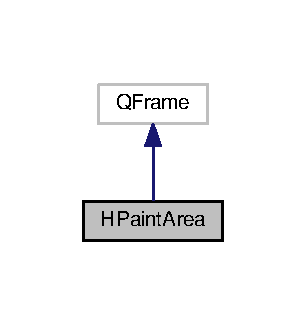
\includegraphics[width=147pt]{class_h_paint_area__inherit__graph}
\end{center}
\end{figure}


H\+Paint\+Area 的协作图\+:\nopagebreak
\begin{figure}[H]
\begin{center}
\leavevmode
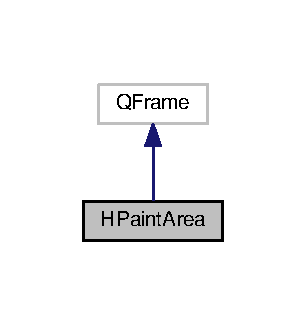
\includegraphics[width=147pt]{class_h_paint_area__coll__graph}
\end{center}
\end{figure}
\subsection*{Public 成员函数}
\begin{DoxyCompactItemize}
\item 
{\bfseries H\+Paint\+Area} (Q\+Widget $\ast$parent=0)\label{class_h_paint_area_a1f22800864c1335ba9a284440d886297}

\item 
void {\bfseries draw\+Outline} (Q\+Painter \&painter)\label{class_h_paint_area_a6888e530cfb3ae1314a6c36c4f5a4e69}

\end{DoxyCompactItemize}


\subsection{详细描述}


在文件 hpaintarea.\+h 第 10 行定义.



该类的文档由以下文件生成\+:\begin{DoxyCompactItemize}
\item 
hpaintarea.\+h\item 
hpaintarea.\+cpp\end{DoxyCompactItemize}

\section{H\+Render\+Controller类 参考}
\label{class_h_render_controller}\index{H\+Render\+Controller@{H\+Render\+Controller}}


类 H\+Render\+Controller 继承关系图\+:\nopagebreak
\begin{figure}[H]
\begin{center}
\leavevmode
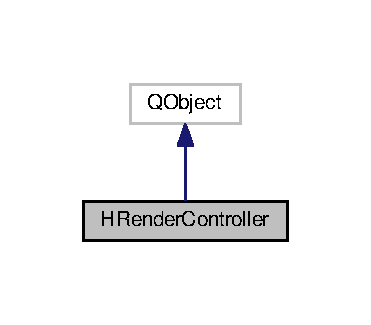
\includegraphics[width=178pt]{class_h_render_controller__inherit__graph}
\end{center}
\end{figure}


H\+Render\+Controller 的协作图\+:\nopagebreak
\begin{figure}[H]
\begin{center}
\leavevmode
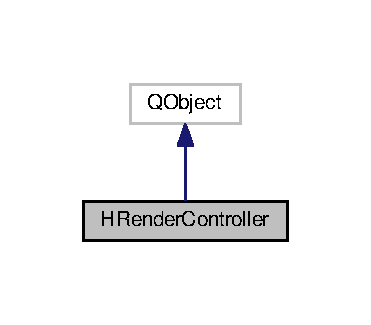
\includegraphics[width=178pt]{class_h_render_controller__coll__graph}
\end{center}
\end{figure}
\subsection*{Public 成员函数}
\begin{DoxyCompactItemize}
\item 
{\bfseries H\+Render\+Controller} (Q\+Widget $\ast$parent, {\bf H\+Document\+Model} $\ast$model)\label{class_h_render_controller_a5210b856b3f8094f63a52a09a6a2c116}

\item 
Q\+Size {\bfseries get\+Parent\+Size} ()\label{class_h_render_controller_a4420f173f24eeca5566e131f21c51c95}

\item 
void {\bfseries render} ()\label{class_h_render_controller_a2d45a5eaa444032f1625f23ed923a349}

\end{DoxyCompactItemize}


\subsection{详细描述}


在文件 hrendercontroller.\+h 第 8 行定义.



该类的文档由以下文件生成\+:\begin{DoxyCompactItemize}
\item 
hrendercontroller.\+h\end{DoxyCompactItemize}

\section{H\+Text\+Cursor类 参考}
\label{class_h_text_cursor}\index{H\+Text\+Cursor@{H\+Text\+Cursor}}


类 H\+Text\+Cursor 继承关系图\+:\nopagebreak
\begin{figure}[H]
\begin{center}
\leavevmode
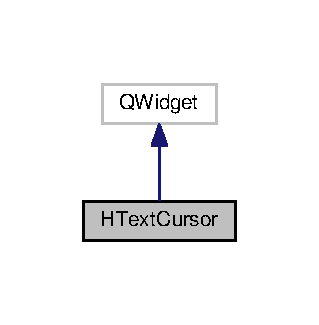
\includegraphics[width=153pt]{class_h_text_cursor__inherit__graph}
\end{center}
\end{figure}


H\+Text\+Cursor 的协作图\+:\nopagebreak
\begin{figure}[H]
\begin{center}
\leavevmode
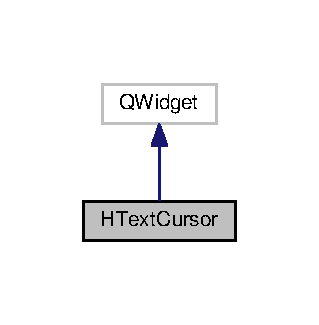
\includegraphics[width=153pt]{class_h_text_cursor__coll__graph}
\end{center}
\end{figure}
\subsection*{Public 槽}
\begin{DoxyCompactItemize}
\item 
void {\bfseries toggle\+Blink} ()\label{class_h_text_cursor_a59202005440d171f2b019ebeae20932d}

\end{DoxyCompactItemize}
\subsection*{Public 成员函数}
\begin{DoxyCompactItemize}
\item 
{\bfseries H\+Text\+Cursor} (Q\+Widget $\ast$parent)\label{class_h_text_cursor_a4c210eb0b6ec5f1e2fcbb451e2388579}

\item 
void {\bfseries set\+Pos} (int, int)\label{class_h_text_cursor_a8a496090b53fb685b8dfbf46d0f0e3c6}

\item 
void {\bfseries set\+Shape} ()\label{class_h_text_cursor_a3c48d99d478a81f5bdd43bad2155b948}

\end{DoxyCompactItemize}


\subsection{详细描述}


在文件 htextcursor.\+h 第 6 行定义.



该类的文档由以下文件生成\+:\begin{DoxyCompactItemize}
\item 
htextcursor.\+h\item 
htextcursor.\+cpp\end{DoxyCompactItemize}

\section{Main\+Window类 参考}
\label{class_main_window}\index{Main\+Window@{Main\+Window}}


类 Main\+Window 继承关系图\+:\nopagebreak
\begin{figure}[H]
\begin{center}
\leavevmode
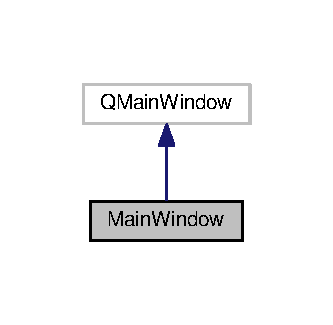
\includegraphics[width=160pt]{class_main_window__inherit__graph}
\end{center}
\end{figure}


Main\+Window 的协作图\+:\nopagebreak
\begin{figure}[H]
\begin{center}
\leavevmode
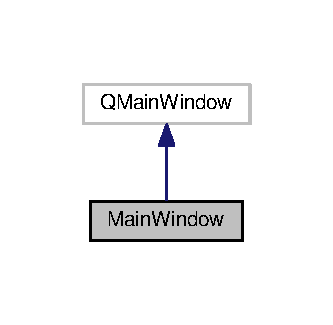
\includegraphics[width=160pt]{class_main_window__coll__graph}
\end{center}
\end{figure}
\subsection*{Public 成员函数}
\begin{DoxyCompactItemize}
\item 
{\bfseries Main\+Window} (Q\+Widget $\ast$parent=0)\label{class_main_window_a8b244be8b7b7db1b08de2a2acb9409db}

\end{DoxyCompactItemize}


\subsection{详细描述}


在文件 mainwindow.\+h 第 11 行定义.



该类的文档由以下文件生成\+:\begin{DoxyCompactItemize}
\item 
mainwindow.\+h\item 
mainwindow.\+cpp\end{DoxyCompactItemize}

%--- End generated contents ---

% Index
\backmatter
\newpage
\phantomsection
\clearemptydoublepage
\addcontentsline{toc}{chapter}{索引}
\printindex

\end{document}
